% mnras_template.tex 
%
% LaTeX template for creating an MNRAS paper
%
% v3.0 released 14 May 2015
% (version numbers match those of mnras.cls)
%
% Copyright (C) Royal Astronomical Society 2015
% Authors:
% Keith T. Smith (Royal Astronomical Society)

% Change log
%
% v3.0 May 2015
%    Renamed to match the new package name
%    Version number matches mnras.cls
%    A few minor tweaks to wording
% v1.0 September 2013
%    Beta testing only - never publicly released
%    First version: a simple (ish) template for creating an MNRAS paper

%%%%%%%%%%%%%%%%%%%%%%%%%%%%%%%%%%%%%%%%%%%%%%%%%%
% Basic setup. Most papers should leave these options alone.
\documentclass[fleqn,usenatbib]{mnras}

% MNRAS is set in Times font. If you don't have this installed (most LaTeX
% installations will be fine) or prefer the old Computer Modern fonts, comment
% out the following line
\usepackage{newtxtext,newtxmath}
% Depending on your LaTeX fonts installation, you might get better results with one of these:
%\usepackage{mathptmx}
%\usepackage{txfonts}

% Use vector fonts, so it zooms properly in on-screen viewing software
% Don't change these lines unless you know what you are doing
\usepackage[T1]{fontenc}

% Allow "Thomas van Noord" and "Simon de Laguarde" and alike to be sorted by "N" and "L" etc. in the bibliography.
% Write the name in the bibliography as "\VAN{Noord}{Van}{van} Noord, Thomas"
\DeclareRobustCommand{\VAN}[3]{#2}
\let\VANthebibliography\thebibliography
\def\thebibliography{\DeclareRobustCommand{\VAN}[3]{##3}\VANthebibliography}


%%%%% AUTHORS - PLACE YOUR OWN PACKAGES HERE %%%%%

% Only include extra packages if you really need them. Common packages are:
\usepackage{graphicx}	% Including figure files
\usepackage{amsmath}	% Advanced maths commands
\usepackage{amssymb}	% Extra maths symbols

%%%%%%%%%%%%%%%%%%%%%%%%%%%%%%%%%%%%%%%%%%%%%%%%%%

%%%%% AUTHORS - PLACE YOUR OWN COMMANDS HERE %%%%%

% Please keep new commands to a minimum, and use \newcommand not \def to avoid
% overwriting existing commands. Example:
%\newcommand{\pcm}{\,cm$^{-2}$}	% per cm-squared

%%%%%%%%%%%%%%%%%%%%%%%%%%%%%%%%%%%%%%%%%%%%%%%%%%

%%%%%%%%%%%%%%%%%%% TITLE PAGE %%%%%%%%%%%%%%%%%%%

% Title of the paper, and the short title which is used in the headers.
% Keep the title short and informative.
\title[Kilonova modeling with SNEC]{Radiation hydrodynamics modeling of kilonovae with SNEC}

% The list of authors, and the short list which is used in the headers.
% If you need two or more lines of authors, add an extra line using \newauthor
\author[Z.~Wu]{
Zhenyu Wu,$^{1}$\thanks{E-mail: 171840687\@smail.nju.edu.cn}
Full author list TBD
\\
% List of institutions
$^{1}$ Nanjing University\\
}

% These dates will be filled out by the publisher
\date{Accepted XXX. Received YYY; in original form ZZZ}

% Enter the current year, for the copyright statements etc.
\pubyear{2021}

% Don't change these lines
\begin{document}
\label{firstpage}
\pagerange{\pageref{firstpage}--\pageref{lastpage}}
\maketitle

% Abstract of the paper
\begin{abstract}
\textcolor{red}{Draft version, not for distribution}
\end{abstract}

% Select between one and six entries from the list of approved keywords.
% Don't make up new ones.
\begin{keywords}
keyword1 -- keyword2 -- keyword3
\end{keywords}

%%%%%%%%%%%%%%%%%%%%%%%%%%%%%%%%%%%%%%%%%%%%%%%%%%%%%%%%%%%%%%%%%%%%%%%%%%%%%

\begin{enumerate}
    \item Use bibtex keys from INSPIRE. I have a script to generate the bibtex automatically from those
    \item The section titles are just suggestions and will be finalized later
    \item Let's start with assembling the relevant plots and some text for the methods section
\end{enumerate}

% ===========================================================================
\section{Introduction}
% ===========================================================================

% ===========================================================================
\section{Methods}
% ===========================================================================
\begin{itemize}
    \item Brief overview of SNEC\\
    SNEC, the SuperNova Explosion Code, is a spherically symmetric (1D) Lagrangian radiation-hydrodynamics code simulating core-collapse supernova explosion. (\cite{morozova2015light}) After reading in the structure and chemical compositions of a progenitor star and the explosion type, the code calculates its explosion and generates bolometric and multicolor light curves. The code mainly uses Paczynski EOS, namely taking into account the ions, electrons and radiation, and solves Saha equations. The code includes radioactive decay of $^{56}$Ni to power supernovae. Rosseland mean opacity is adopted for radiation transfer. 
    
    Unlike core-collapse supernovae, kilonovae are powered by radioactive decay of heavy elements synthesis through r-process. Modeling the opacities of r-process elements and the heating rates due to their decay is the key to kilonova simulations. Given the complexity of elements in kilonovae, we use the average properties of different compositions, like the initial electron fraction $Y_e$. Moreover, the intial profiles of supernova progenitors in SNEC are from MESA, while we use two kinds of profiles here. We use wind profiles for code validation and comparison with other analytical models. We also have more realistic initial profiles derived from numerical relativity. In the following we will explain the opacities, heating rates, initial and boundary conditions in our code and other differences from SNEC.
    

    \item Opacities\\
     Tanaka et al has done detailed research on opacities of mixture of r-process elements. In (\cite{tanaka2018properties}),  they show that bolometric lightcurves with grey opacity of $1.0$ cm$^2$ g$^{-1}$ and $10.0$ cm$^2$ g$^{-1}$ agree with results using wavelength-dependent radiative transfer. The grey opacity values were also adopted for red, purple and blue kilonova components in (\cite{villar2017combined}) to fit AT2017gfo. In our model, we use grey opacity and set its lower and upper bound to $1.0$ cm$^2$ g$^{-1}$ and $10.0$ cm$^2$ g$^{-1}$ respectively. We set the opacity corresponding to $Y_e \ 0.25$ to the intermediate $5.5$ cm$^2$ g$^{-1}$, and then use a simple smooth function to describe the change of opacity $\kappa$ with $Y_e$:
        
    
    \begin{equation}
    	\label{opacity_ye}
    	\kappa = 1 + \frac{9}{1+(4Y_e)^{12}}~~ \mathrm{ [cm^2 g^{-1}]}
    \end{equation}
    
    Figure \ref{opacity_Ye} shows the comparison of our model with (\cite{tanaka2020systematic}) results. It is worth noting that, for simplicity, the opacity in our model is a constant, namely it doesn't change with time or temperature. In addition, grey opacity's application to multicolor light curves needs further study.
   
    
    \begin{figure}
    \centering
    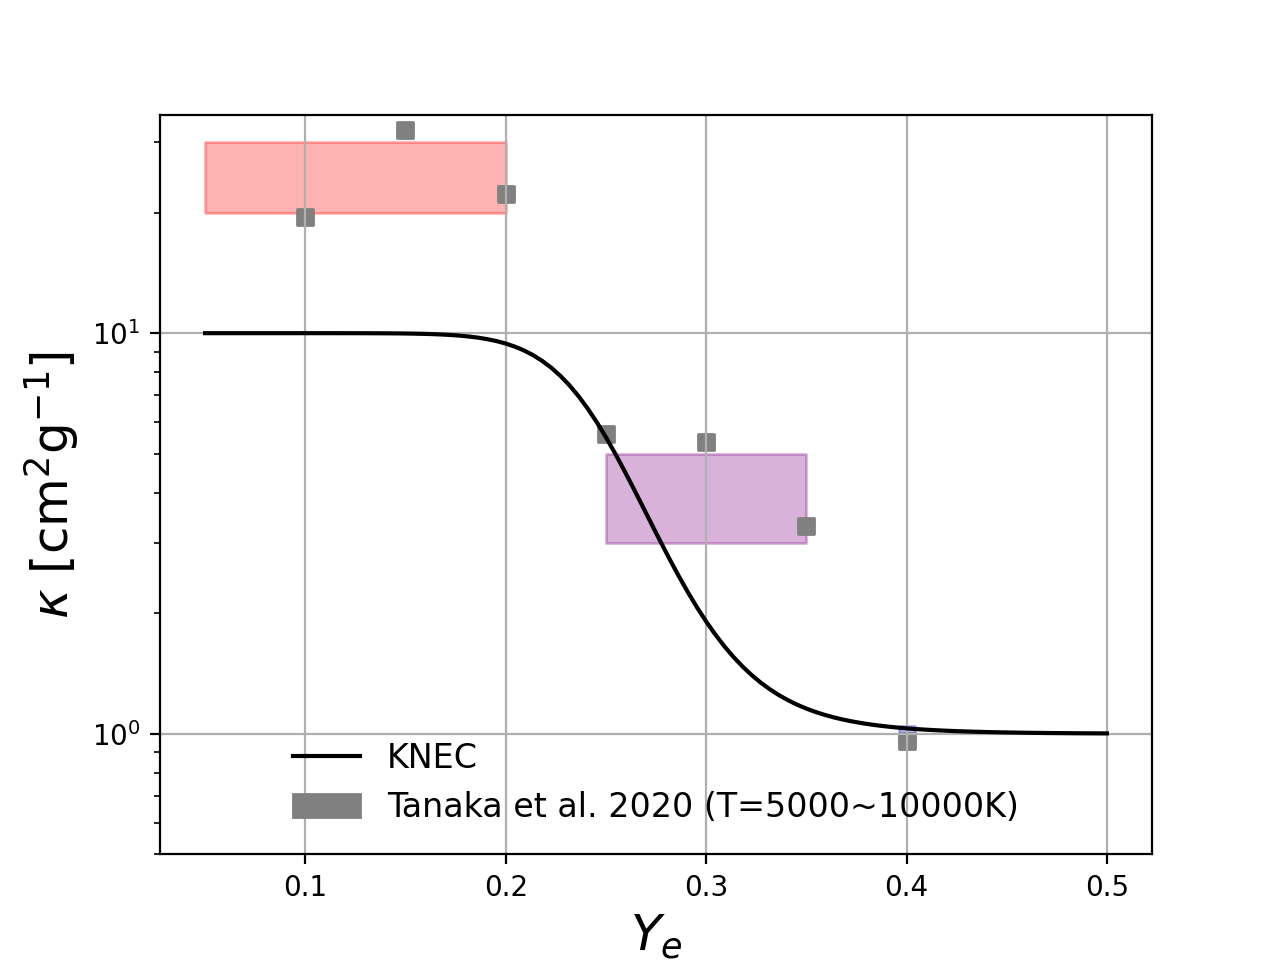
\includegraphics[scale=0.5]{figures/opacity_Ye.png}
    \caption{The solid line is opacity as a function of $Y_e$ in our model  (Equation \ref{opacity_Ye}). Little grey squares show Tanaka et al's data, and the large rectangles are the suggested opacity range in their paper. (at 5000 $\sim$ 10000K, and they decrease steeply at lower temperature.) Opacity in our model is a little lower than their results due to the upper bound $10$ cm$^2$ g$^{-1}$ we set.}
    \label{opacity_Ye}
    \end{figure} 
    


    
    
    
    \item Heating rates\\
    At the times relevant for kilonovae, the ejecta has already lost all of its initial thermal energy at expansion, and the dominant source of heating is constituted by the decays of heavy elements produced in the r-process. This heating can be described by a specific heating rate which can be derived by evolving the system of the numerous characteristic nuclides in time while accounting for their mutual interactions.\\
    Here, time-dependent heating rates obtained using the nuclear reaction network SkyNet with a FRDM nuclear mass model are employed. A single SkyNet run is determined by the set of thermodynamic variables initial electron fraction $Y_e$, initial specific entropy $s$ and expansion timescale $\tau$. The rates are thus computed on a comprehensive grid with $0.02\leq Y_e\leq0.48$ linearly spaced, $1.82$ $\mathrm{k_B/baryon}$ $\leq s\leq100$ $\mathrm{k_B/baryon}$ and $1.36$ ms $\leq\tau\leq100$ ms log-spaced, the results on a representative subgrid being reported in Figure \ref{heatrates}.\\
    \begin{figure}
    \centering
    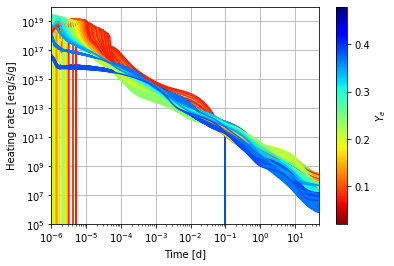
\includegraphics[scale=0.6]{figures/heating/heating rate fits/heatrates.png}
    \caption{Heating rate trajectories as obtained by SkyNet on a subgrid of thermodynamic variables $0.05\leq Y_e\leq0.4$, $3$ $\mathrm{k_B/baryon}$ $\leq s\leq50$ $\mathrm{k_B/baryon}$ and $1$ ms $\leq\tau\leq30$ ms for visual clarity. Trajectories are color-coded to indicate different initial electron fractions. Vertical lines correspond to SkyNet noise which is averaged out in the fit procedure.}
    \label{heatrates}
    \end{figure}
    In order to derive the heating rate for arbitrary initial conditions, the above trajectories are reduced to a parametrized functional form by means of a fit procedure intended to cover the time interval from $0.1$ s to $50$ days post-merger, and, in particular, a distinction between time regimes is introduced. For early times $t\lesssim0.1$ days, the analytic fitting formula, derived from detailed nucleosynthesis calculations (\cite{Korobkin:2012uy}), is employed:
    \begin{equation}
    \label{eqKorfit}
    \dot{\epsilon}_{\mathrm{r}}(t)=\epsilon_0\epsilon_{\mathrm{th}}\left(\frac{1}{2}-\frac{1}{\pi}\arctan{\left[\frac{t-t_0}{\sigma}\right]}\right)^{\alpha},
    \end{equation}
    where $\epsilon_0$, $\alpha$, $t_0$ and $\sigma$ are considered fit parameters, while $\epsilon_{\mathrm{th}}<1$ is the thermalization efficiency. At late times $t\gtrsim0.1$ days instead, we expect a power-law fit to be a sufficiently good approximation of the heating rates, and thus the fitting formula becomes:
    \begin{equation}
    \label{eqpowfit}
    \dot{\epsilon}_{\mathrm{r}}(t)=\epsilon_0'\epsilon_{\mathrm{th}}t^{-\alpha'},
    \end{equation}
    with $\epsilon_0'$ and $\alpha'$ additional fit parameters. The heating rate fits, as obtained by using equations \ref{eqKorfit} and \ref{eqpowfit}, are then joint together with a log-scaled smoothing procedure applied on the time interval $1\times10^3$ s $\leq t\leq4\times10^4$ s, centered on $t\sim0.1$ days in log-scale.\\
    Figure \ref{heatratesfit} shows the fitted version of the heating rate trajectories presented in Figure \ref{heatrates}.
    \begin{figure}
    \centering
    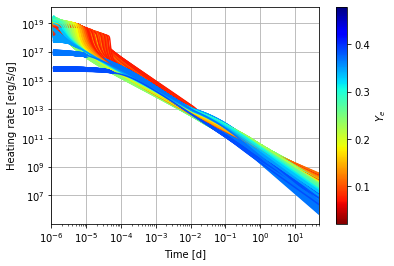
\includegraphics[scale=0.65]{figures/heating/heating rate fits/heatratesfit.png}
    \caption{Heating rate fitted trajectories as obtained by performing the fit procedure on a subgrid of thermodynamic variables $0.05\leq Y_e\leq0.4$, $3$ $\mathrm{k_B/baryon}$ $\leq s\leq50$ $\mathrm{k_B/baryon}$ and $1$ ms $\leq\tau\leq30$ ms for visual clarity. Trajectories are color-coded to indicate different initial electron fractions.}
    \label{heatratesfit}
    \end{figure}
    The quality of a single fit is evaluated using a mean fractional log error, defined as:
    \begin{equation}
    \label{eqlogerror}
    \Delta(\dot{\epsilon}_{\mathrm{r}})=\left<\frac{|\ln(\dot{\epsilon}_{\mathrm{r}}^o(t))-\ln(\dot{\epsilon}_{\mathrm{r}}(t))|}{\ln(\dot{\epsilon}_{\mathrm{r}}^o(t))}\right>,
    \end{equation}
    where $\dot{\epsilon}_{\mathrm{r}}^o(t)$ is the original SkyNet heating rate trajectory, and the mean is performed over the entire time window $0.1$ s $\leq t\leq50$ days. As visible in Figure \ref{fiterror}, our fit procedure returns considerably accurate results: the vast majority of trajectories are reproduced within $\sim1\%$ relative error, while the worst cases, corresponding to external points in the input grid, carry only a slightly higher error $\lesssim 5\%$.
    \begin{figure}
    \centering
    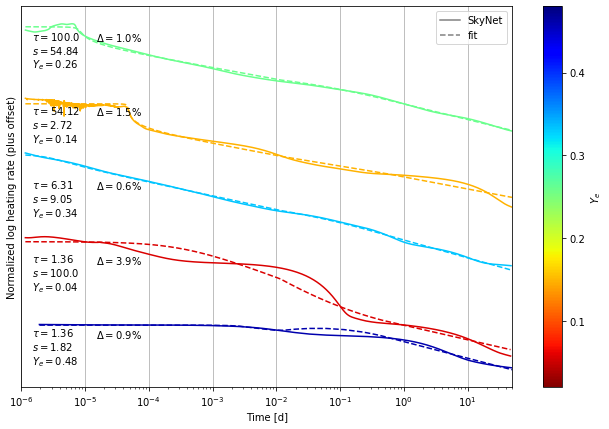
\includegraphics[scale=0.4]{figures/heating/heating rate fits/fiterror.png}
    \caption{Heating rate SkyNet trajectory along with its fitted version for five different representative sets of thermodynamic variables. Each fit is matched with its relative error defined by equation \ref{eqlogerror}. Trajectories are color-coded to indicate different initial electron fractions.}
    \label{fiterror}
    \end{figure}
    
    
    \item Initial and boundary conditions
    \item Other differences from SNEC
    \item Bolometric luminosities and Multicolor luminosities
\end{itemize}

% ===========================================================================
\section{Code validation}
% ===========================================================================
\subsection{Hydrodynamics}
\subsection{Energy conservation}

The energy conservation equation in hydrodynamics is 

 \begin{equation}
 \label{conservation_1}
 \begin{aligned}
 	 	\frac{\mathrm{d}}{\mathrm{d} t} \int_{\Omega} \rho\left(\epsilon+\frac{1}{2} \boldsymbol{v}^{2}\right) \mathrm{d} V & =\int_{\Omega} \rho \boldsymbol{f_b} \cdot \boldsymbol{v} \mathrm{~d} V -\int_{\partial \Omega} p \boldsymbol{v} \cdot \mathrm{d} \boldsymbol{S} \\&-\int_{\partial \Omega} \boldsymbol{f_s} \cdot \mathrm{d} \boldsymbol{S}+\int_{\Omega} \rho q \mathrm{~d}V
 \end{aligned}
 \end{equation}
 
 Here the surface force $\boldsymbol{f_s}$ = 0 and the body force $\boldsymbol{f_b}$ is the gravitational force. $\epsilon$ represents specific internal energy and $q$ is the heating term including r-process heating and radiation. Therefore, we can write energy conservation as
 



\begin{equation}
\label{conservation_2}
	\frac{d}{dt}(E_{int} + E_{kin}+E_{grav}) = \dot Q - \int p \boldsymbol{v} \cdot d \boldsymbol{S} 
\end{equation}
$\dot Q = H - L_{bol}$, $H$ is the heating from decay of r-process elements and $L_{bol}$ is the bolometric luminosity. For $p_{imax}=0$ boundary condition, the pdV term $-\int p \boldsymbol{v} \cdot d \boldsymbol{S} = p_{1} dV = p_{1} v_1 4\pi r_1^2$  
Integrate Equation (\ref{conservation_2}) over time, we have cumulative energy conservation shown in Figure \ref{energy_conservation}.
 

\begin{figure}
\centering
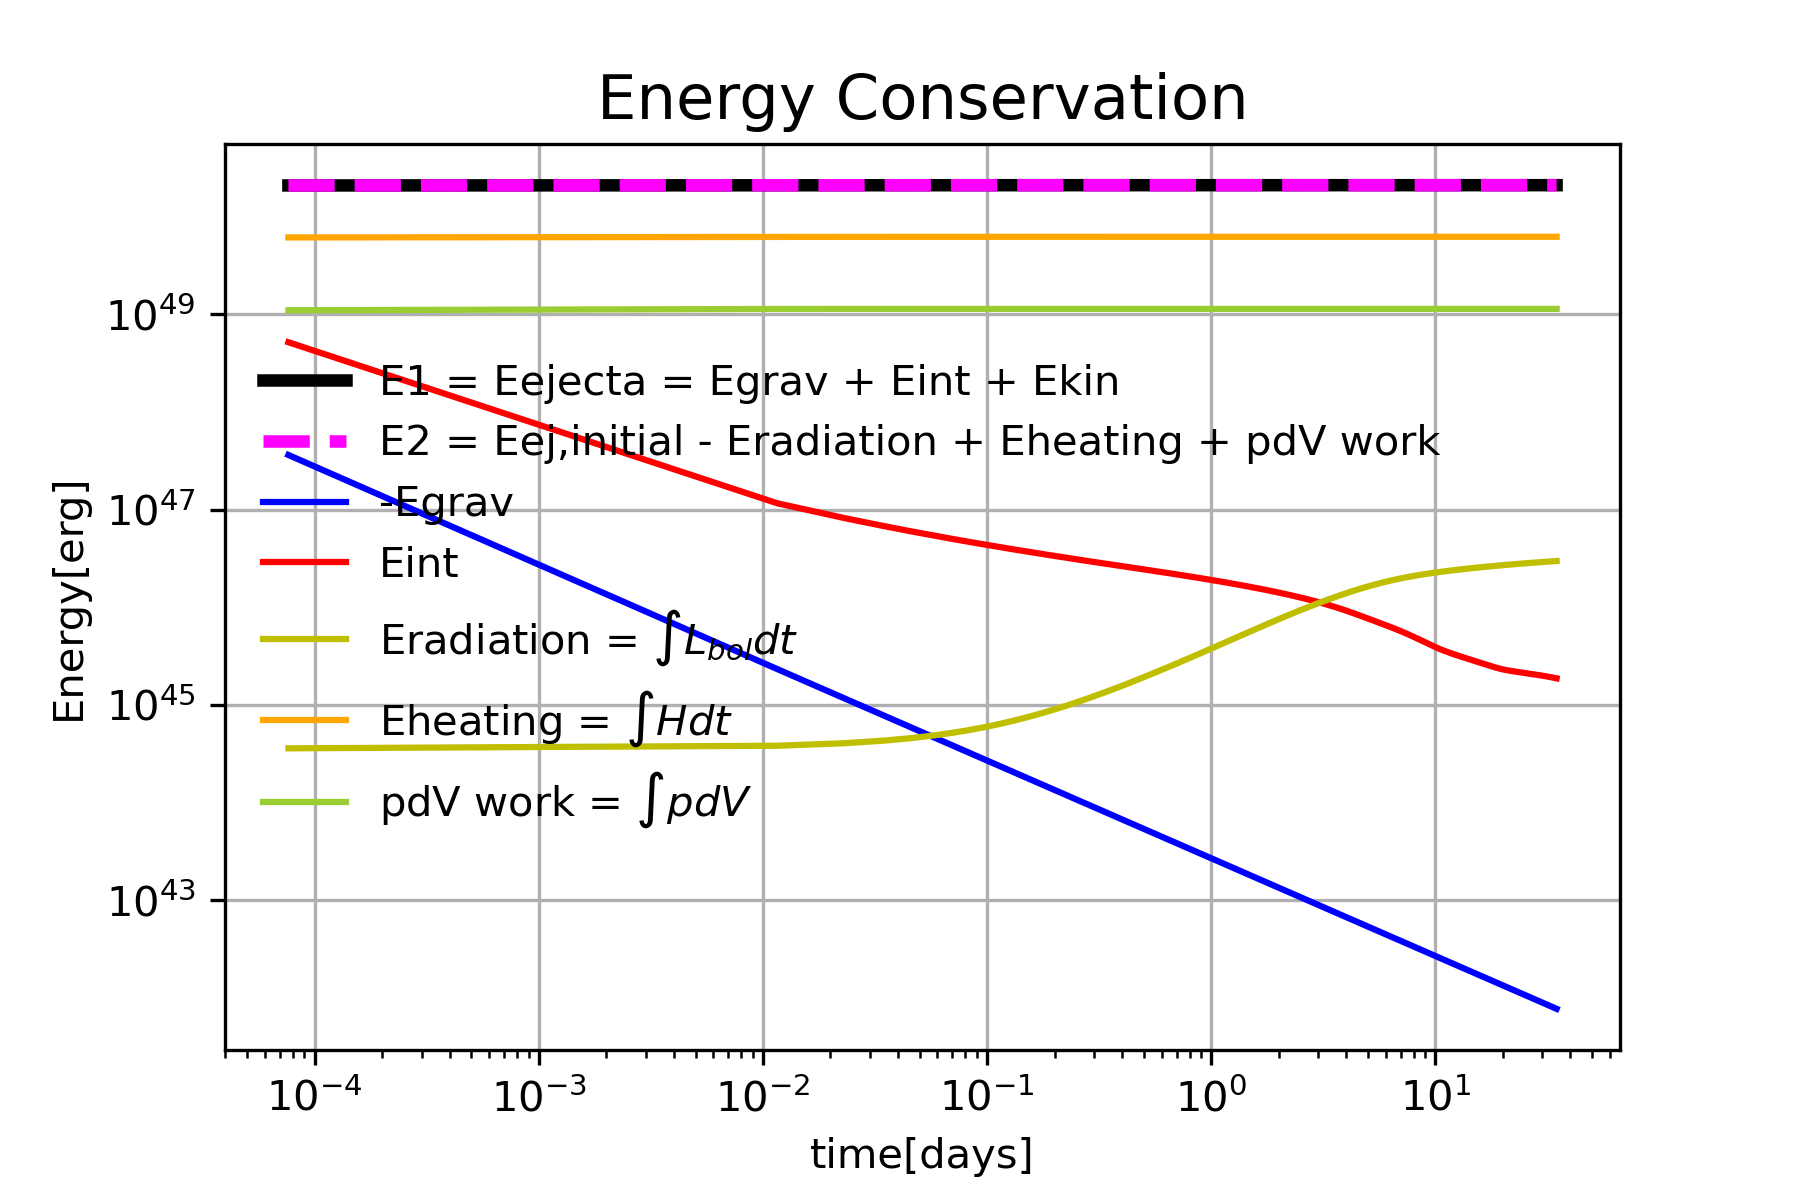
\includegraphics[scale=0.6]{figures/energy_conservation_wind3_Apr2.png}
\caption{Energy conservation of wind3 ejecta ($0.01M_{\odot}, v_{max}=0.2c, Y_e=0.05, s=10\ \mathrm{k_B}, \tau=10\ \mathrm{ ms}$), using $p_{imax}=0$ boundary condition. $E_1$ is the total energy of the ejecta, $E_2$ is the initial ejecta energy + energy from heating - luminosity + pdV work at inner boundary. The maximum difference between $E_1$ and $E_2$ is 0.015\%.}
\label{energy_conservation}
\end{figure}



\subsection{Comparison with analytic models}

% ===========================================================================
\section{Ab-initio simulations: from mergers to kilonovae}
% ===========================================================================
\subsection{General features}
\subsection{Impact of uncertainties in the heating rates}

% ===========================================================================
\section{A first application to AT2017gfo}
% ===========================================================================
\subsection{Best fitting analytical models}
\subsection{Comparison between NR informed models and observations}
\subsection{Impact of shock cooling}

% ===========================================================================
\section{Conclusions}
% ===========================================================================

\bibliographystyle{mnras}
\bibliography{references}


% Don't change these lines
\bsp	% typesetting comment
\label{lastpage}
\end{document}

% End of mnras_template.tex
